
\documentclass[12pt,a4paper]{report}
\usepackage[a4paper,left=1.25in,right=1in,top=1in,bottom=1in]{geometry}
\usepackage{mathptmx}
\usepackage{graphicx}
\usepackage{setspace}
\usepackage{fancyhdr}
\IfFileExists{titlesec.sty}{\usepackage{titlesec}}{}
\IfFileExists{tocloft.sty}{\usepackage{tocloft}}{}
\usepackage{array}
\usepackage{booktabs}
\usepackage{longtable}
\usepackage{caption}
\IfFileExists{enumitem.sty}{\usepackage{enumitem}}{}
\usepackage[hidelinks]{hyperref}
\usepackage{ragged2e}

\graphicspath{{figures/}{../docs/}}
\setstretch{1.12}
\setlength{\parindent}{0pt}
\setlength{\parskip}{5pt}
\justifying
\renewcommand{\contentsname}{TABLE OF CONTENTS}
\renewcommand{\listfigurename}{LIST OF FIGURES}
\renewcommand{\listtablename}{LIST OF TABLES}
\captionsetup{font=bf,labelfont=bf,justification=centering}
\renewcommand{\thefigure}{\thechapter.\arabic{figure}}
\renewcommand{\thetable}{\thechapter.\arabic{table}}
\renewcommand{\figurename}{Fig.}
\setcounter{tocdepth}{0}

\makeatletter
\@ifpackageloaded{tocloft}{
\renewcommand{\cftchapfont}{\normalfont}
\renewcommand{\cftchappagefont}{\normalfont}
\renewcommand{\cftdotsep}{1}
\renewcommand{\cftfigpresnum}{Fig. }
\setlength{\cftfignumwidth}{0.75in}
\renewcommand{\cfttabpresnum}{Table }
\setlength{\cfttabnumwidth}{0.9in}
}{}
\@ifpackageloaded{titlesec}{
\titleformat{\chapter}{\normalfont\bfseries\centering\fontsize{16}{19}\selectfont}{CHAPTER \thechapter}{0.5em}{\MakeUppercase}
\titlespacing*{\chapter}{0pt}{0pt}{16pt}
\titleformat{name=\chapter,numberless}{\normalfont\bfseries\centering\fontsize{16}{19}\selectfont}{}{0pt}{\MakeUppercase}
\titleformat{\section}{\normalfont\bfseries\fontsize{14}{17}\selectfont}{\thesection}{3em}{\MakeUppercase}
\titleformat{\subsection}{\normalfont\bfseries\fontsize{12}{15}\selectfont}{\thesubsection}{3em}{}
}{}
\makeatother

\newcommand{\studentid}{23AIML010}
\newcommand{\chapterheader}{CHAPTER HEADING}
\fancyhf{}
\fancyhead[L]{\fontsize{10}{12}\selectfont\studentid}
\fancyhead[R]{\fontsize{10}{12}\selectfont\chapterheader}
\fancyfoot[L]{\fontsize{10}{12}\selectfont CSPIT, CHARUSAT}
\fancyfoot[C]{\fontsize{10}{12}\selectfont\thepage}
\fancyfoot[R]{\fontsize{10}{12}\selectfont Department of Artificial Intelligence and Machine Learning}
\renewcommand{\headrulewidth}{0pt}
\renewcommand{\footrulewidth}{0pt}
\newcommand{\frontchapter}[1]{\chapter*{#1}\addcontentsline{toc}{chapter}{#1}\markboth{#1}{#1}}

\begin{document}
\pagestyle{empty}
\pagenumbering{gobble}
\begin{titlepage}
\thispagestyle{empty}
\begin{singlespace}
\centering

\includegraphics[width=3.5in]{charusat_logo.png}\par
\vspace{0.15in}
{\bfseries\fontsize{16}{19}\selectfont A SUMMER INTERNSHIP REPORT\par}
\vspace{0.10in}
{\bfseries\fontsize{14}{17}\selectfont ON\par}
\vspace{0.10in}
{\bfseries\fontsize{16}{19}\selectfont ECOROUTE SYSTEM / ECOROUTE ENGINE\par}
\vspace{0.14in}
{\bfseries Geospatial Fleet Routing and Dispatch Optimization Platform\par}
\vspace{0.14in}
Prepared by\par
{\bfseries\fontsize{14}{17}\selectfont OM CHIRAGBHAI CHOKSI\par}
{\bfseries 23AIML010\par}
\vspace{0.13in}
Under the guidance of\par
{\bfseries [Internal Guide Name]\par}
[Designation]\par
\vspace{0.13in}
Submitted to Charotar University of Science and Technology\par
Degree of Bachelor of Technology in\par
{\bfseries Artificial Intelligence and Machine Learning\par}
\vspace{0.11in}
{\bfseries Summer Internship Project\par}
Internship Organization: Logicwind\par
Duration: Six months ongoing, started from 1 June 2026\par
Current status: one month completed and five months remaining\par
\vspace{0.14in}
Submitted at\par
{\bfseries Department of Artificial Intelligence and Machine Learning\par}
{\bfseries Chandubhai S. Patel Institute of Technology (CSPIT)\par}
Faculty of Technology and Engineering, CHARUSAT\par
Changa, Dist. Anand - 388421\par
\vspace{0.08in}
{\bfseries July 2026\par}
\end{singlespace}
\end{titlepage}

\chapter*{Certificate}
This is to certify that the Summer Internship report entitled ``EcoRoute System / EcoRoute Engine'' is a bonafide work carried out by OM CHIRAGBHAI CHOKSI (23AIML010), student of B.Tech Artificial Intelligence and Machine Learning, under academic guidance during the Summer Internship Project at Chandubhai S. Patel Institute of Technology (CSPIT), CHARUSAT.

The internship at Logicwind is planned for six months. This report documents the first completed month of internship learning, backend engineering exposure, codebase study and project implementation work. To the best of my knowledge, the work presented in this report is satisfactory for interim academic internship documentation.

\vspace{1.35in}
\begin{center}
\begin{tabular}{p{0.45\textwidth}p{0.45\textwidth}}
\centering\rule{2.3in}{0.4pt} & \centering\arraybackslash\rule{2.3in}{0.4pt}\\
\centering Internal Guide & \centering\arraybackslash Head of Department
\end{tabular}
\end{center}
\clearpage

\chapter*{Company / Organization Certificate}
The company or organization certificate should be inserted on this page as provided by Logicwind. Since the internship is still ongoing, the final certificate may be issued after completion of the full six-month internship period.

\vspace{2.0in}
\begin{center}\bfseries [Insert official company certificate here]\end{center}
\clearpage

\chapter*{Declaration by the Candidate}
I hereby declare that the internship report entitled ``EcoRoute System / EcoRoute Engine'' submitted by me to Chandubhai S. Patel Institute of Technology (CSPIT), CHARUSAT, is a record of bonafide internship learning and project work carried out during my summer internship at Logicwind.

I further declare that this report represents the first completed month of a six-month ongoing internship. The remaining five months are still in progress, and therefore this report does not claim final completion of the full internship period.

\vspace{0.8in}
\begin{flushright}
\rule{2.2in}{0.4pt}\\
OM CHIRAGBHAI CHOKSI\\
23AIML010
\end{flushright}
\clearpage

\pagestyle{fancy}
\pagenumbering{roman}
\setcounter{page}{1}
\renewcommand{\chapterheader}{PRELIMINARY PAGES}
\frontchapter{Acknowledgement}
I express my sincere gratitude to Logicwind for providing me the opportunity to work in a professional backend development environment. The first month of internship helped me observe how real software tasks are planned, assigned, reviewed and improved through disciplined engineering workflow.

I am thankful to my company mentors and senior team members for guidance in backend architecture, API design, database design, security practices, code review and project documentation. I also thank my internal guide [Internal Guide Name], the Department of Artificial Intelligence and Machine Learning, CSPIT and CHARUSAT for academic support and encouragement.

This report also refers to the formatting sequence and front-matter style of the Bhumi reference DOCX, while adapting the content for my AIML department, CSPIT context and EcoRoute backend project.
\clearpage

\frontchapter{Abstract}
EcoRoute System, also known as EcoRoute Engine, is a geospatial fleet routing and dispatch optimization backend for waste collection, recycling logistics and circular economy transportation. The system focuses on organization-scoped operational workflows such as business management, pickup requests, vehicle management, driver assignment, dispatch automation, route generation, audit logging, notifications and dashboard metrics.

This report presents my first-month learning during an ongoing six-month internship at Logicwind. The inspected codebase contains a TypeScript and Express.js backend, PostgreSQL/PostGIS database schema, OSRM routing client, Swagger/OpenAPI documentation, Docker Compose support, Jest/Supertest tests and a Next.js frontend. The report describes the project GitHub repository, file structure, database schema, database tables, API flow, security flow, routing integration, testing strategy and learning outcomes. Mermaid reference diagrams are stored as \texttt{.mmd} files and rendered as rich figures for inclusion in the PDF report. GraphQL and Apollo Server are included as internship learning topics, but the EcoRoute implementation itself is REST and OpenAPI based.
\clearpage

\begingroup
\small
\setstretch{0.80}
\tableofcontents
\endgroup
\clearpage
\listoffigures
\clearpage
\listoftables
\clearpage

\frontchapter{Description of Company / Organization}
Logicwind is a software development organization where I received practical exposure to backend development and professional project workflow. During the first month, I learned how tasks are discussed, split into smaller responsibilities, tracked through ClickUp and reviewed by senior developers. This helped me understand that production backend work requires clarity, disciplined implementation and good communication.

The internship is planned for six months. This report records the first completed month only, so the observations are intentionally written as interim learning and project progress. The remaining five months will provide more time for deeper backend contribution and stronger ownership.
\clearpage

\pagenumbering{arabic}
\setcounter{page}{1}
\renewcommand{\chapterheader}{CHAPTER 1}
\chapter{Introduction}
\section{Background of Internship}
Summer internship training connects academic learning with practical software development. As a B.Tech Artificial Intelligence and Machine Learning student at CSPIT, I used this opportunity to understand backend engineering in a real project environment. Although my academic branch is AIML, the internship helped me see how AI-oriented applications still depend on strong backend foundations such as APIs, databases, authentication, deployment and maintainable architecture.

\section{Project Context}
EcoRoute System is a backend-centered platform for fleet routing and dispatch in waste collection and recycling logistics. The project is useful because logistics operations need reliable assignment of pickup requests to vehicles, route planning using road network data and operational visibility through dashboards and audit logs.

The project repository is available at: \url{https://github.com/OMCHOKSI108/ecoroute-system}. The local repository inspected for this report contains backend, frontend, database, documentation, testing and report folders.

\section{Objectives and Scope}
The objective of the first month was to understand professional backend development and study the EcoRoute codebase deeply. The scope includes REST API design, JWT authentication, RBAC, Zod validation, PostgreSQL/PostGIS schema design, OSRM routing, Docker-based setup, Swagger documentation, testing and report preparation.
\clearpage

\renewcommand{\chapterheader}{CHAPTER 2}
\chapter{Literature and Technology Background}
\section{Backend Engineering Background}
Modern logistics systems require scalable APIs, consistent database updates and clear separation of concerns. A layered backend helps achieve these goals by separating route definitions, request validation, controller handling, service-level business rules and repository-level database access. This makes the system easier to test and modify.

\section{Geospatial and Routing Background}
EcoRoute uses PostgreSQL with PostGIS to store location-aware records such as business addresses, pickup locations and vehicle locations. PostGIS geography columns and GiST indexes support efficient spatial lookup paths. OSRM provides routing services such as nearest road matching, distance matrix calculation and route/trip computation using OpenStreetMap-derived road networks.

\section{REST, GraphQL and Apollo Learning}
The EcoRoute project is implemented using REST APIs documented through OpenAPI and Swagger UI. During the internship, I also studied GraphQL and Apollo Server as learning topics. GraphQL uses schema definitions, queries, mutations and resolvers, while REST usually exposes resource-specific endpoints. This comparison helped me understand API design trade-offs.
\clearpage

\renewcommand{\chapterheader}{CHAPTER 3}
\chapter{System Analysis}
\section{Functional Requirements}
The system must support organization-scoped users, authentication, businesses, pickup locations, waste categories, vehicles, drivers, pickup requests, dispatch assignment, route generation, route stop tracking, notifications, audit logs and dashboard metrics. It must also expose health and routing endpoints for operational readiness and map-based workflows.

\begin{table}[h!]
\centering
\caption{Functional Requirements of EcoRoute System}
\begin{tabular}{|p{1.8in}|p{3.6in}|}
\hline
\textbf{Requirement Area} & \textbf{Description}\\ \hline
Authentication & Register, login, token refresh, logout, forgot password and reset password workflows.\\ \hline
Business and Pickups & Manage businesses, pickup locations, waste categories and pickup request lifecycle.\\ \hline
Fleet and Dispatch & Manage vehicles, drivers, vehicle status, dispatch preview, manual assignment and auto assignment.\\ \hline
Routing & Generate route records, route stops, route geometry, distance and estimated duration.\\ \hline
Operations & Provide dashboard metrics, notifications, vehicle location tracking and audit logs.\\ \hline
\end{tabular}
\end{table}

\section{Non-Functional Requirements}
Important non-functional requirements include security, maintainability, reliability, portability and performance. The project uses JWT, RBAC, request validation, database constraints, transactions, Docker Compose and test automation to support these qualities.

\begin{table}[h!]
\centering
\caption{Non-Functional Requirements of EcoRoute System}
\begin{tabular}{|p{1.8in}|p{3.6in}|}
\hline
\textbf{Quality Attribute} & \textbf{Implementation Direction}\\ \hline
Security & JWT access control, role checks, password hashing, CORS, Helmet and rate limiting.\\ \hline
Reliability & Transactional dispatch updates, row locks, constraints and consistent error handling.\\ \hline
Maintainability & Layered modules, TypeScript types, Zod schemas and repository isolation.\\ \hline
Performance & Spatial indexes, database indexes and local OSRM routing support.\\ \hline
Portability & Docker Compose, environment variables and offline routing stubs.\\ \hline
\end{tabular}
\end{table}
\clearpage

\renewcommand{\chapterheader}{CHAPTER 4}
\chapter{Technology Stack}
\section{Tools and Technologies Used}
The technology stack was identified from the backend and frontend package files, Docker files, migrations and source code. The backend uses Node.js, Express.js and TypeScript. PostgreSQL and PostGIS are used for data persistence and spatial support. Swagger/OpenAPI documents APIs, and Jest/Supertest support testing.

\begin{table}[h!]
\centering
\caption{Technology Stack Summary}
\begin{tabular}{|p{1.5in}|p{3.9in}|}
\hline
\textbf{Area} & \textbf{Technologies / Practices}\\ \hline
Backend & Node.js, Express.js, TypeScript, routes, controllers, services and repositories.\\ \hline
Database & PostgreSQL, PostGIS, SQL migrations, indexes, constraints and transactions.\\ \hline
Frontend & Next.js, React, dashboard pages, dispatch components and API hooks.\\ \hline
Security & JWT, RBAC middleware, bcrypt hashing, Helmet, CORS and rate limiting.\\ \hline
Documentation & OpenAPI, Swagger UI, README files, screenshots and Mermaid references.\\ \hline
Testing and DevOps & Jest, Supertest, Postman collection, Docker, Docker Compose and Git.\\ \hline
\end{tabular}
\end{table}

\begin{figure}[h!]
\centering
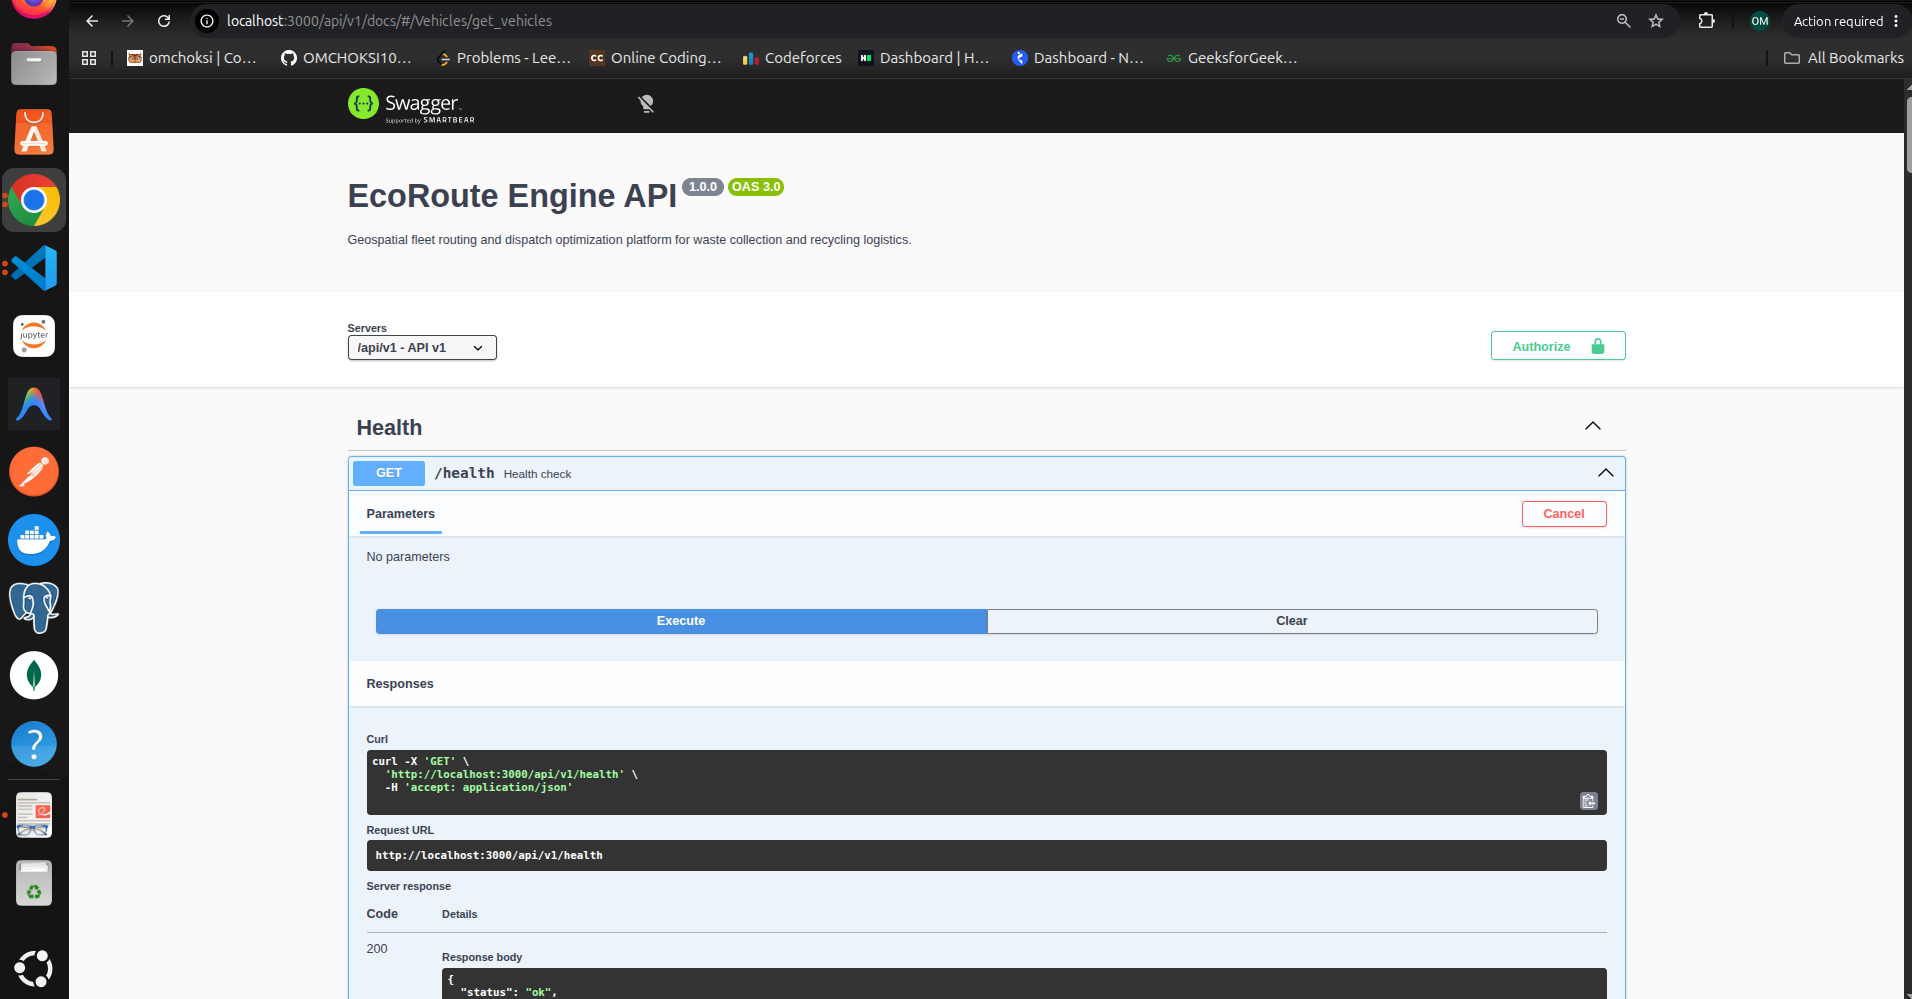
\includegraphics[width=0.86\textwidth]{backend_swagger.png}
\caption{EcoRoute Backend Swagger Documentation UI}
\end{figure}
\clearpage

\renewcommand{\chapterheader}{CHAPTER 5}
\chapter{System Design}
\section{High-Level Architecture}
EcoRoute follows a layered system design where client applications communicate with the Express API. Security middleware validates identity and role access before request data reaches controllers and services. Services implement business rules and call repositories for database operations or the OSRM client for routing calculations.

\begin{figure}[h!]
\centering
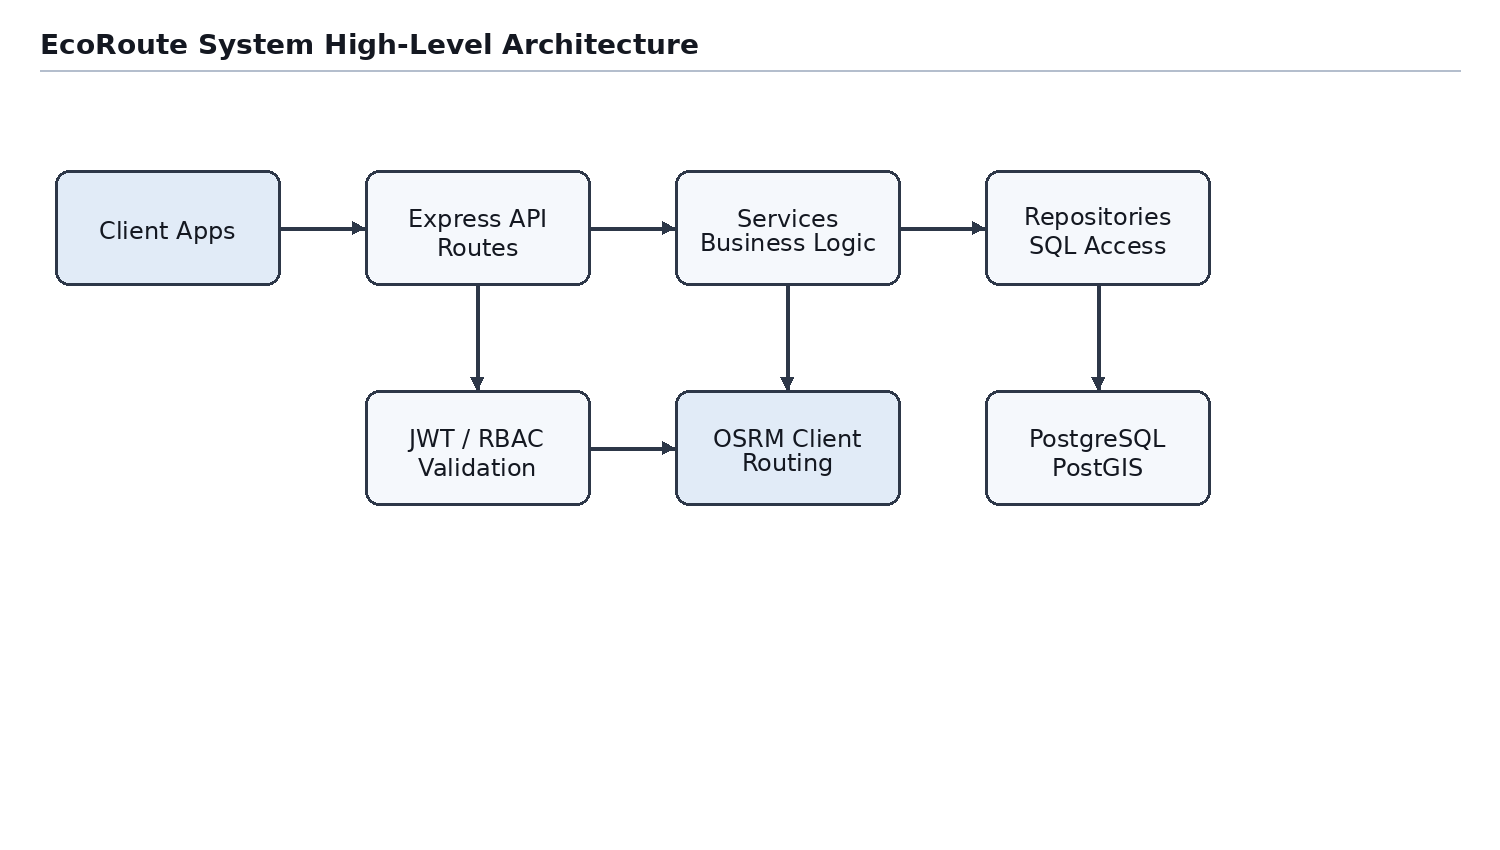
\includegraphics[width=0.88\textwidth]{architecture_high_level.png}
\caption{High-Level Mermaid-Style Architecture of EcoRoute System}
\end{figure}

\section{Layered Backend Architecture}
The layered backend design separates HTTP routing, controllers, schemas, services, repositories and integrations. This structure matches professional backend practice because it keeps controllers thin and places business logic inside services.

\begin{figure}[h!]
\centering
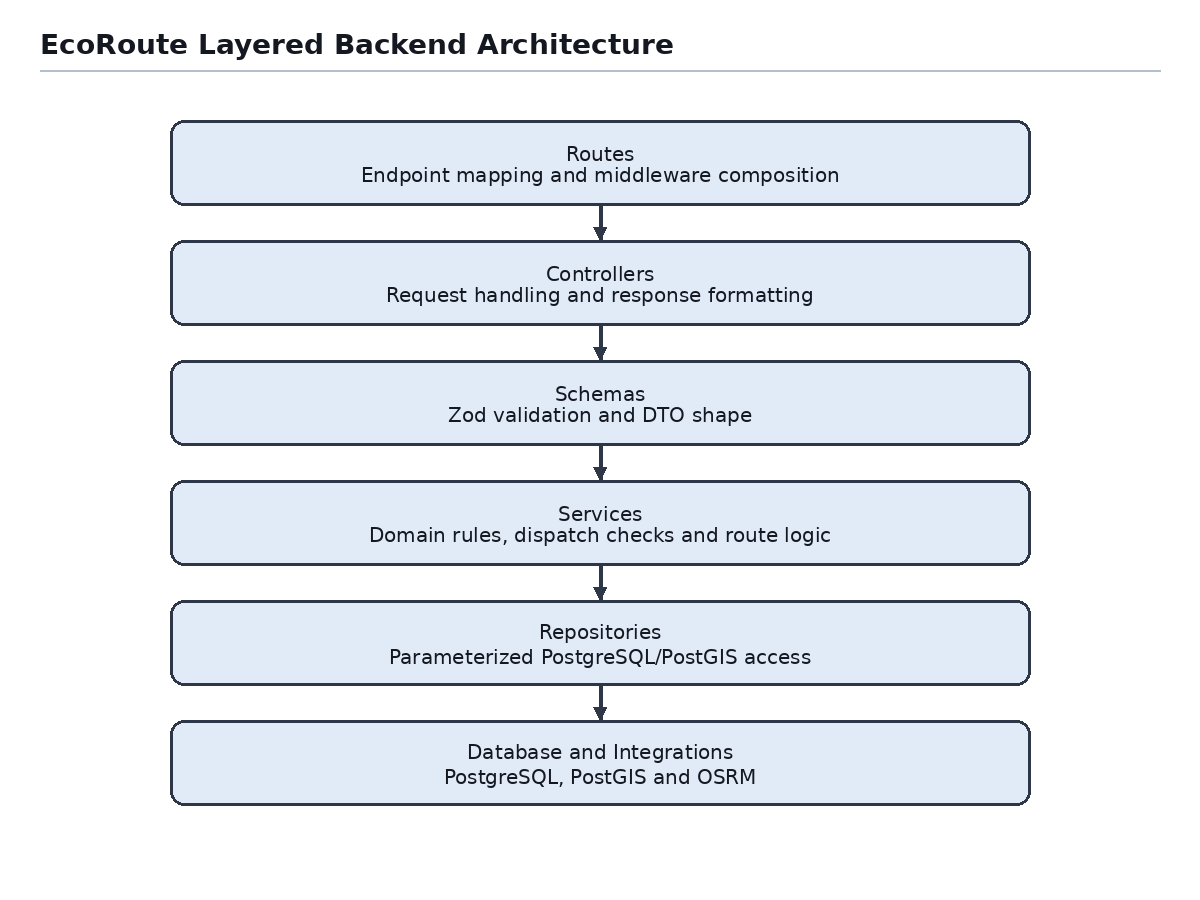
\includegraphics[width=0.78\textwidth]{architecture_layered.png}
\caption{Layered Backend Architecture}
\end{figure}
\clearpage

\section{API Request Lifecycle}
The API lifecycle starts from a client request and passes through Express routing, middleware, validation, controller handling, service processing and repository database access. The response is returned as structured JSON.

\begin{figure}[h!]
\centering
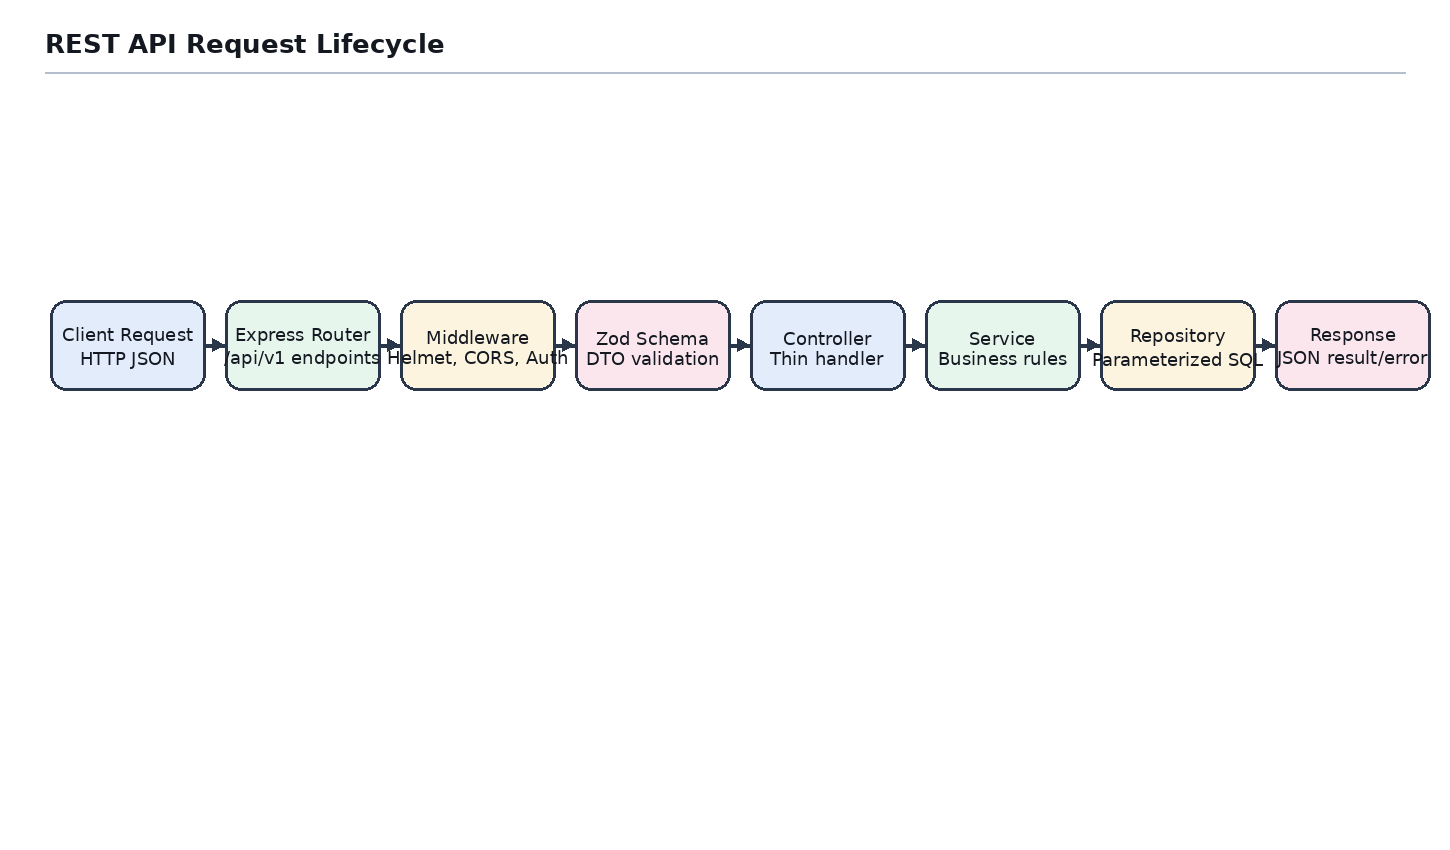
\includegraphics[width=0.90\textwidth]{api_request_lifecycle.png}
\caption{REST API Request Lifecycle}
\end{figure}

\section{Frontend and Backend Integration}
The frontend folder contains a Next.js application with pages for dashboard, dispatch, vehicles, pickups, routes, drivers, users, organizations and notifications. Hooks and API client utilities connect the frontend to backend REST endpoints.

\begin{figure}[h!]
\centering
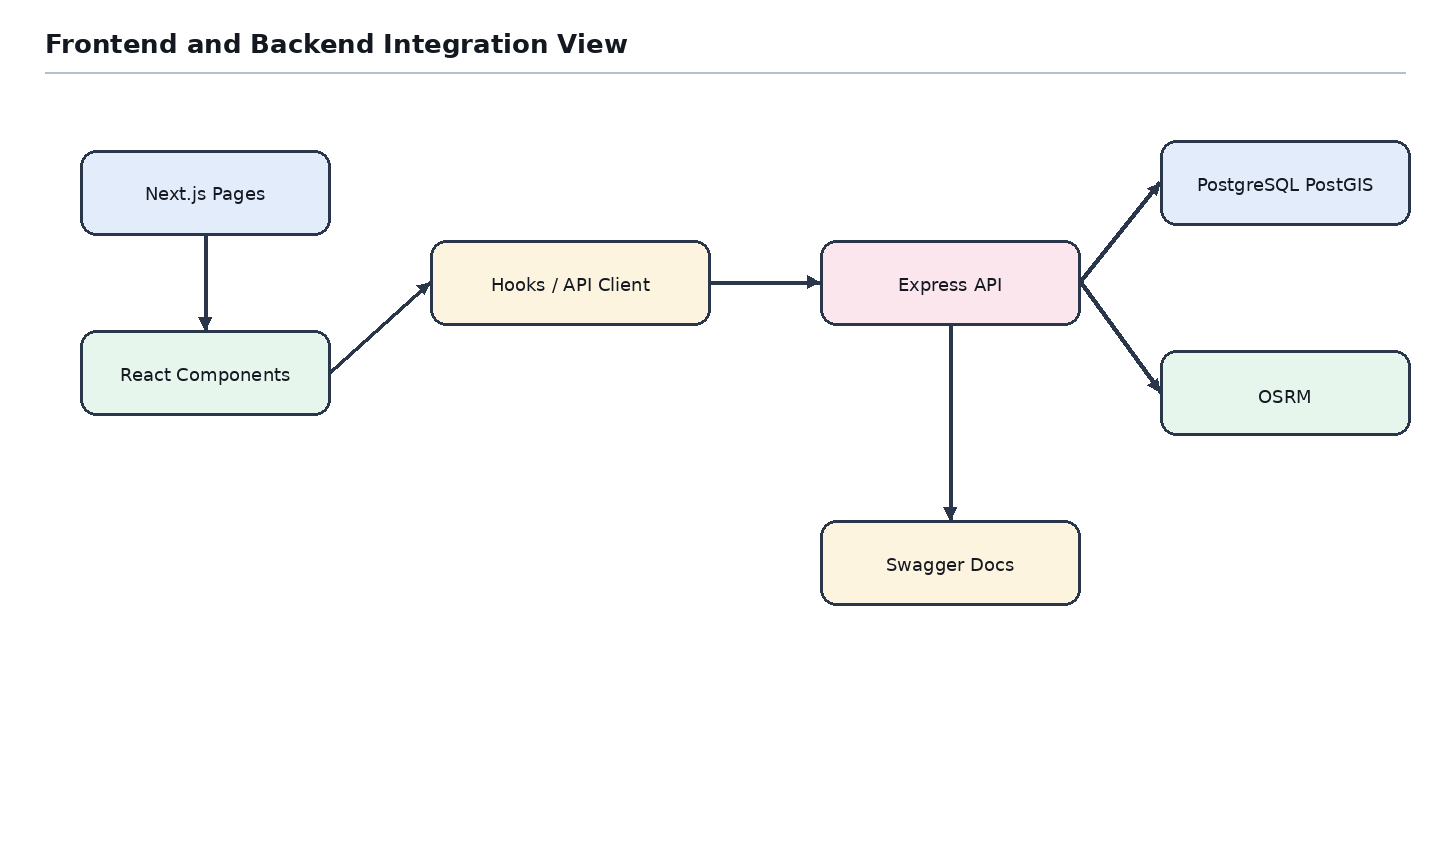
\includegraphics[width=0.88\textwidth]{frontend_backend_integration.png}
\caption{Frontend and Backend Integration View}
\end{figure}
\clearpage

\renewcommand{\chapterheader}{CHAPTER 6}
\chapter{Project File Structure and Database Design}
\section{Project File Structure}
The repository is organized into backend, frontend, docs, testing and report areas. The backend follows a modular structure, while the frontend contains Next.js pages and reusable components.

\begin{figure}[h!]
\centering
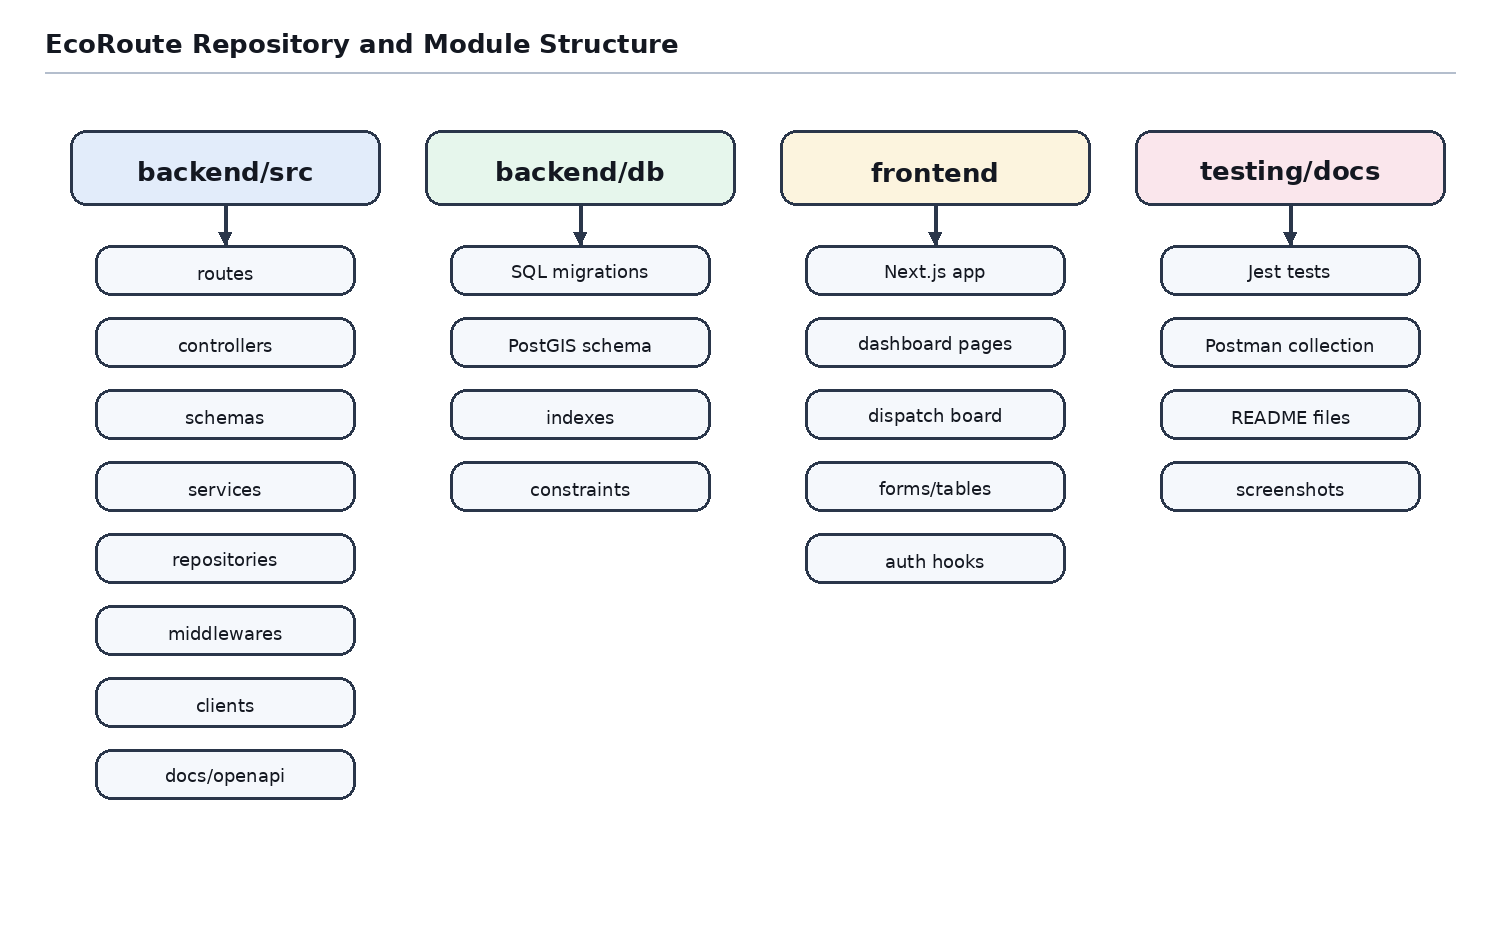
\includegraphics[width=0.86\textwidth]{repository_structure.png}
\caption{EcoRoute Repository and Module Structure}
\end{figure}

\begin{verbatim}
ecoroute_system/
  backend/src/
    routes/ controllers/ schemas/ services/ repositories/
    middlewares/ clients/ config/ docs/ types/
  backend/db/migrations/
    001_auth.sql ... 008_password_reset_otps.sql
  frontend/app/
    dashboard/ dispatch/ vehicles/ pickups/ routes/ drivers/
  frontend/components/
    auth/ dashboard/ dispatch/ vehicles/ pickups/ routes/ ui/
  docs/
    project.md backend_swagger.png backend_running.png
  testing/
    Postman collection and test run output
\end{verbatim}

\section{Database Schema Overview}
The database schema is defined through SQL migrations. It includes identity tables, business data tables, fleet tables, operational routing tables and observability tables. Foreign keys enforce relationships and indexes support lookup performance.

\begin{figure}[h!]
\centering
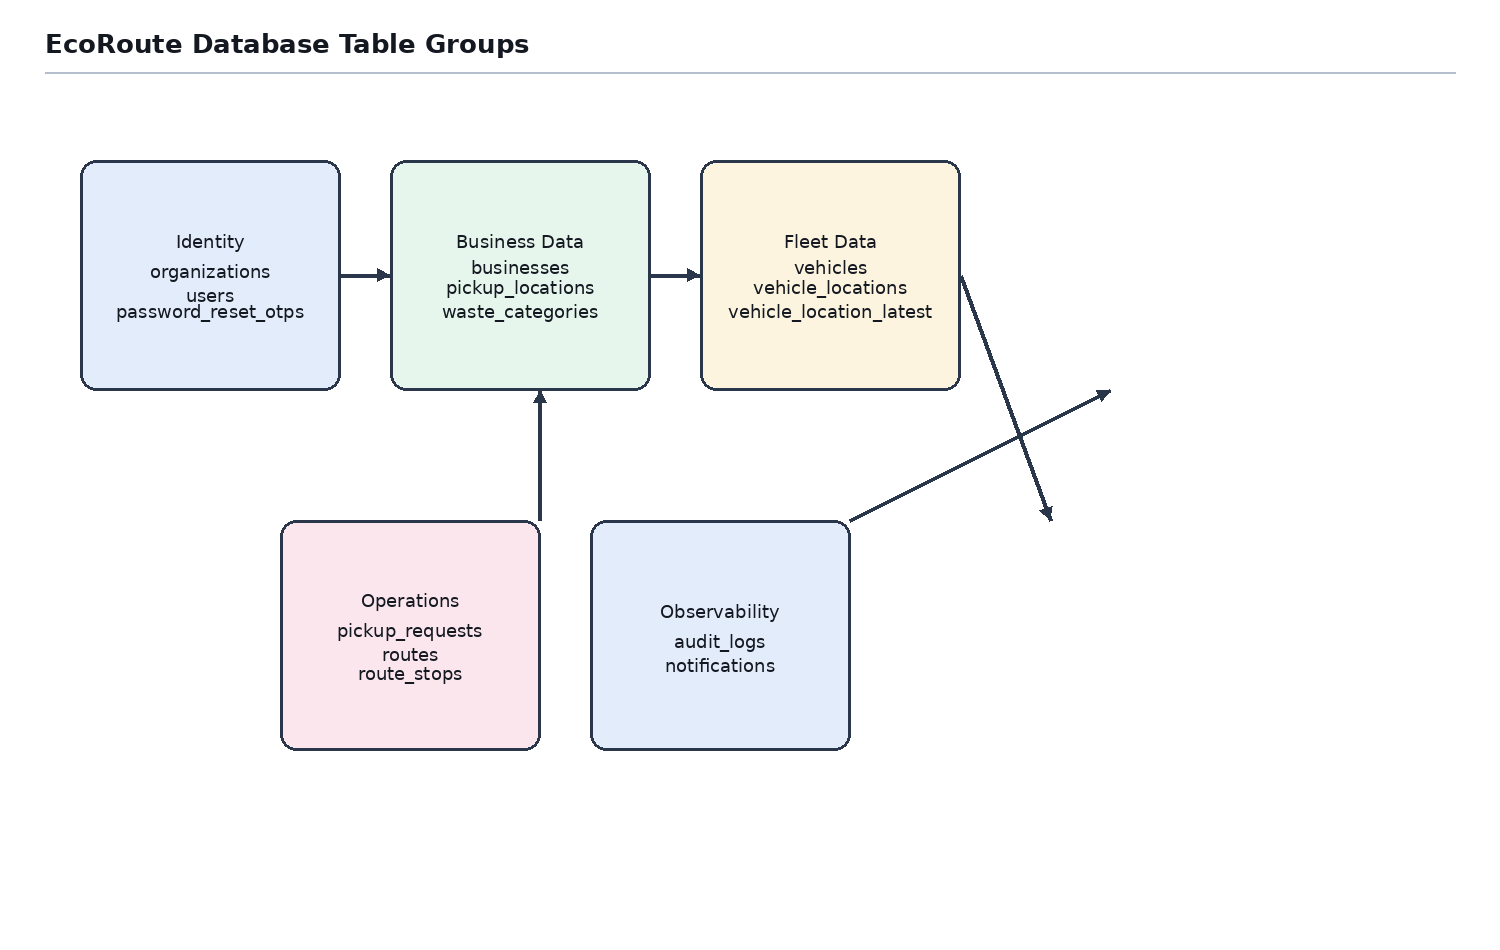
\includegraphics[width=0.84\textwidth]{database_table_groups.png}
\caption{EcoRoute Database Table Groups}
\end{figure}
\clearpage

\begin{longtable}{|p{1.5in}|p{3.9in}|}
\caption{Major Database Tables and Purpose}\\ \hline
\textbf{Table} & \textbf{Purpose}\\ \hline
\endfirsthead
\hline
\textbf{Table} & \textbf{Purpose}\\ \hline
\endhead
organizations & Stores organization records for multi-tenant separation.\\ \hline
users & Stores user accounts, roles, password hashes and active status.\\ \hline
password\_reset\_otps & Stores hashed OTP records for password reset workflow.\\ \hline
businesses & Stores waste/recycling business profiles and geospatial address data.\\ \hline
pickup\_locations & Stores multiple pickup points for each business with PostGIS location.\\ \hline
waste\_categories & Stores organization-scoped waste category records.\\ \hline
vehicles & Stores vehicle capacity, load, status and driver assignment data.\\ \hline
pickup\_requests & Stores pickup lifecycle, assignment and estimated weight data.\\ \hline
routes & Stores generated route records, status, distance, duration and geometry.\\ \hline
route\_stops & Stores ordered route stops and stop-level status.\\ \hline
vehicle\_locations & Stores historical vehicle location reports.\\ \hline
vehicle\_location\_latest & Stores latest vehicle location for fast lookup.\\ \hline
notifications & Stores user notifications and read status.\\ \hline
audit\_logs & Stores operational activity trail for dispatch and other actions.\\ \hline
\end{longtable}
\clearpage

\renewcommand{\chapterheader}{CHAPTER 7}
\chapter{Implementation Details}
\section{Authentication and Authorization}
Authentication uses JWT bearer tokens. The middleware verifies the token and attaches the user payload to the request. Role-based authorization checks whether the user has permission to access protected operations. This design prevents unauthorized users from performing dispatch, route, audit or administrative actions.

\begin{figure}[h!]
\centering
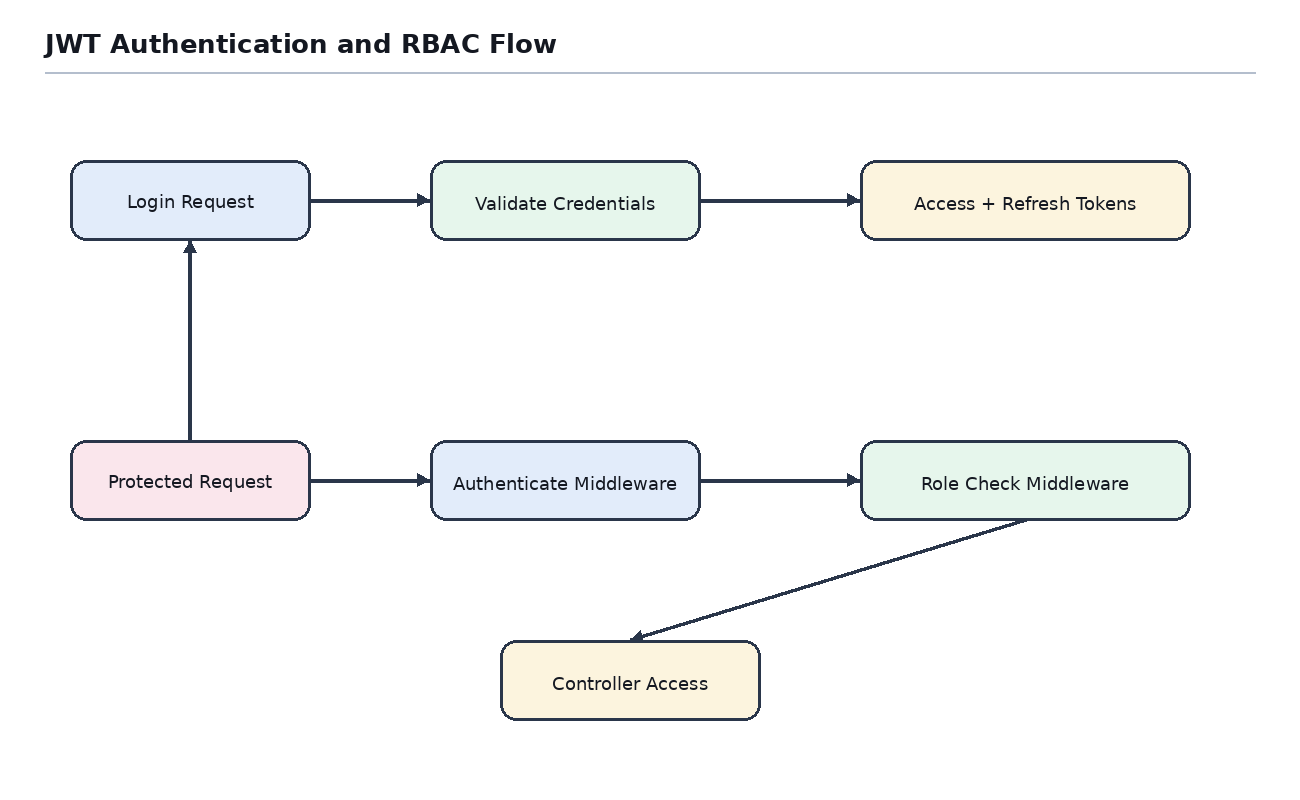
\includegraphics[width=0.82\textwidth]{auth_rbac_flow.png}
\caption{JWT Authentication and RBAC Flow}
\end{figure}

\section{Dispatch Implementation}
The dispatch service supports preview, manual assignment and automatic assignment. For manual assignment, the service opens a transaction, locks the vehicle row, locks pickup rows, validates pickup status, checks capacity, updates vehicle load, assigns pickups and writes an audit log. This protects the system from duplicate assignment and capacity overflow.

\begin{figure}[h!]
\centering
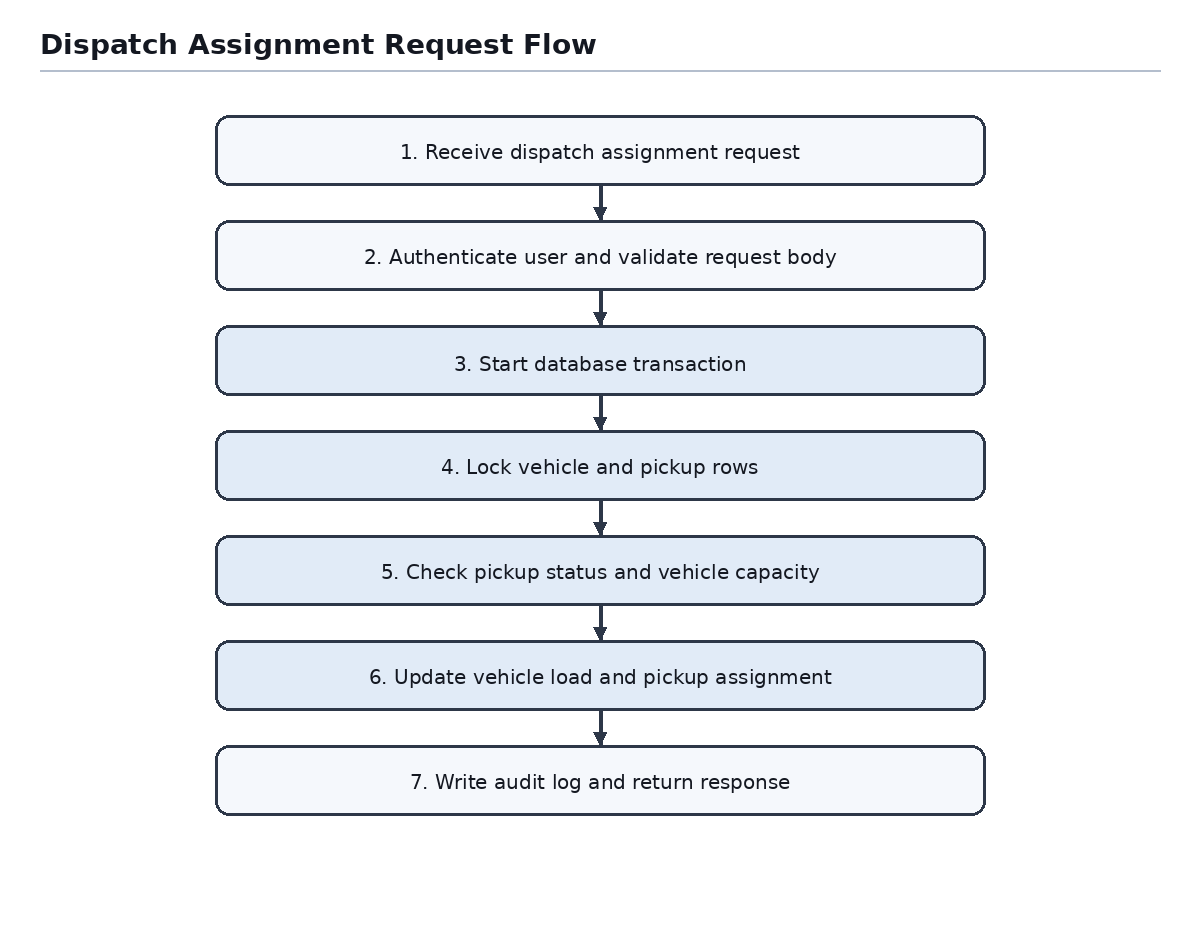
\includegraphics[width=0.82\textwidth]{dispatch_request_flow.png}
\caption{Dispatch Assignment Request Flow}
\end{figure}
\clearpage

\section{Routing and OSRM Integration}
The OSRM client supports nearest, table and trip operations. The implementation handles timeout-bound HTTP calls and also supports offline stubs when external APIs are disabled. This makes local testing easier and prevents unit tests from depending on live routing services.

\begin{figure}[h!]
\centering
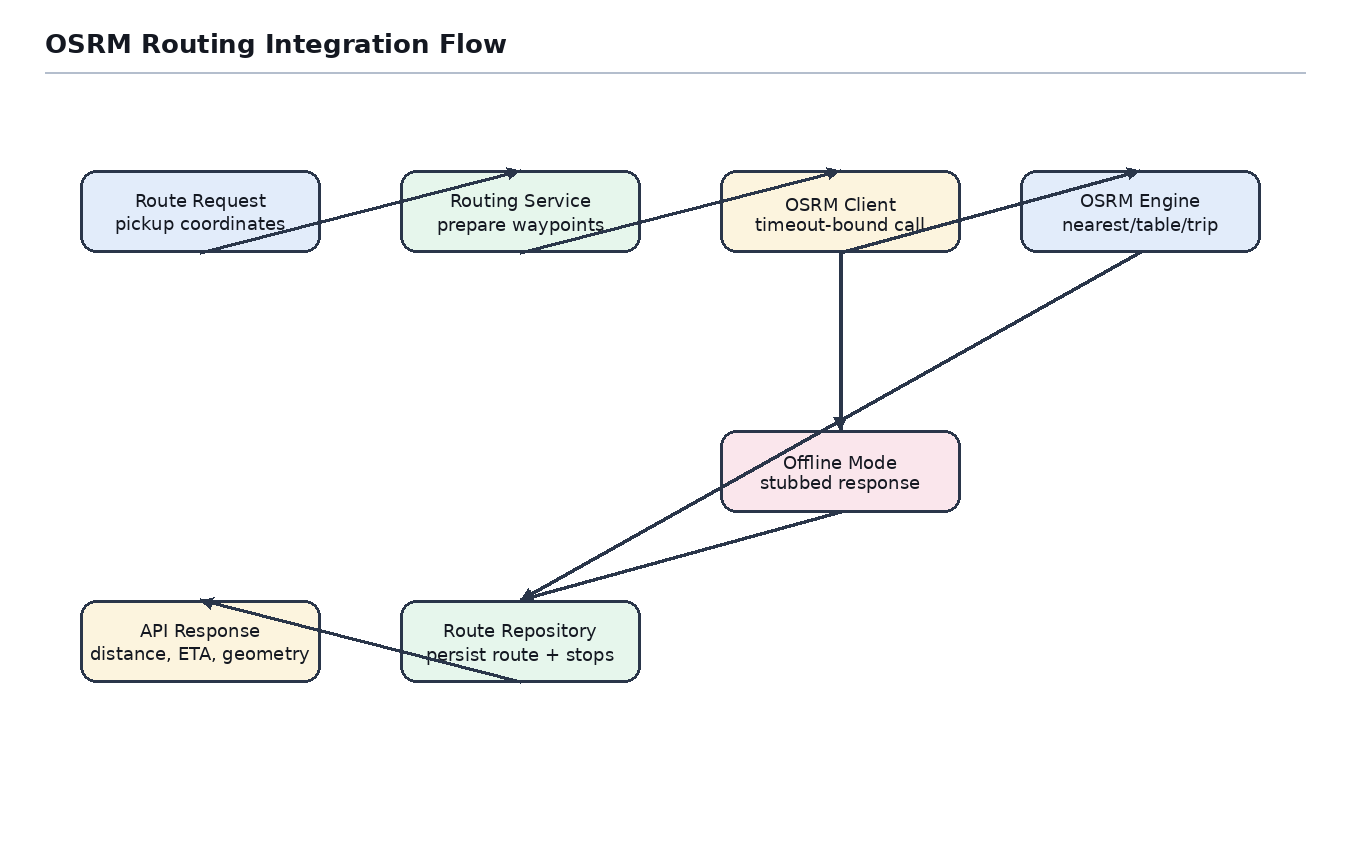
\includegraphics[width=0.84\textwidth]{osrm_routing_flow.png}
\caption{OSRM Routing Integration Flow}
\end{figure}

\section{Docker Deployment View}
Docker Compose defines services for the backend, PostGIS database and migration runner. OSRM is documented as an optional service that requires pre-processed map data. This deployment approach supports local development and portable setup.

\begin{figure}[h!]
\centering
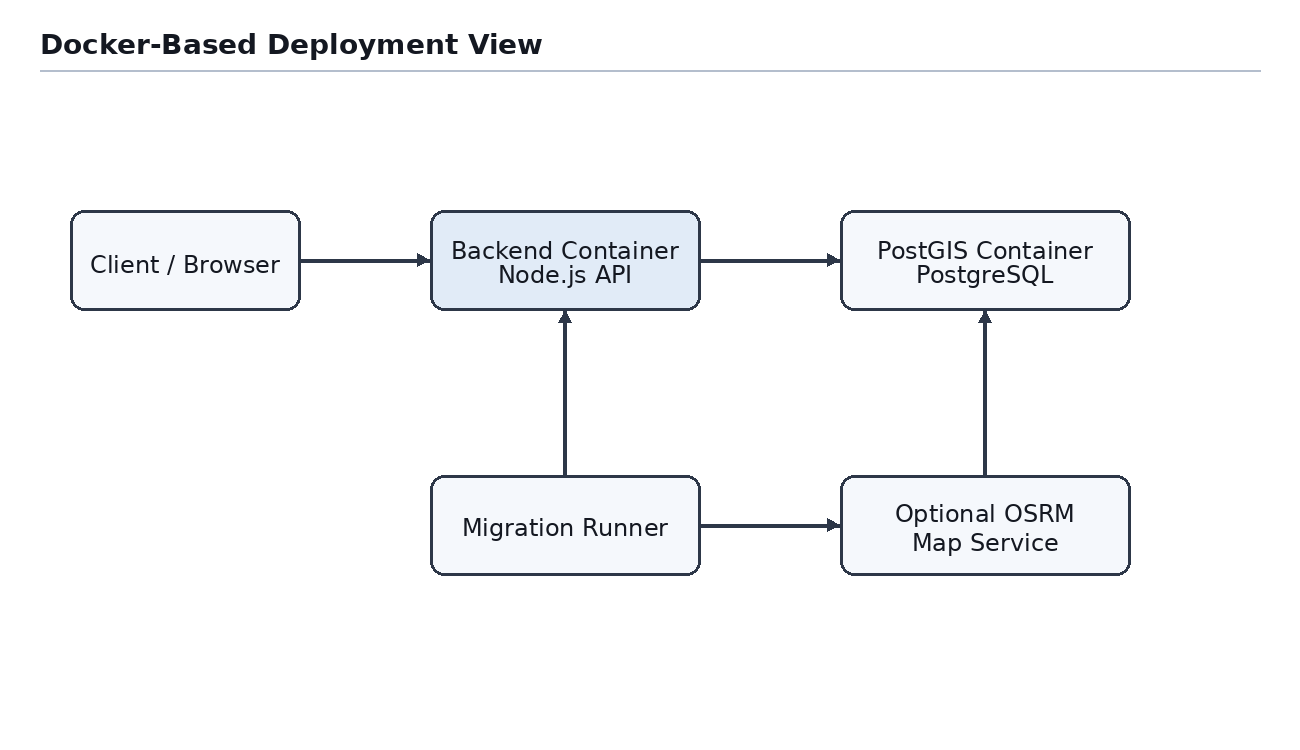
\includegraphics[width=0.80\textwidth]{docker_deployment.png}
\caption{Docker-Based Deployment View}
\end{figure}
\clearpage

\renewcommand{\chapterheader}{CHAPTER 8}
\chapter{Testing and Verification}
\section{Testing Strategy}
The backend contains Jest and Supertest tests for health, authentication, businesses, vehicles, pickups, dispatch, routes, dashboard and audit modules. Tests are important because dispatch and routing workflows include business rules that should not be changed accidentally.

\begin{table}[h!]
\centering
\caption{Testing and Verification Summary}
\begin{tabular}{|p{1.6in}|p{3.8in}|}
\hline
\textbf{Area} & \textbf{Verification Focus}\\ \hline
Authentication & Registration, login, token refresh and protected access behaviour.\\ \hline
Dispatch & Capacity validation, duplicate assignment prevention and transactional updates.\\ \hline
Routes and Routing & Route generation, OSRM stubs and route-state consistency.\\ \hline
Dashboard and Audit & Metrics endpoints, operational audit trail and organization-scoped data.\\ \hline
Health and Docs & Health endpoint readiness and Swagger/OpenAPI documentation availability.\\ \hline
\end{tabular}
\end{table}

\begin{figure}[h!]
\centering
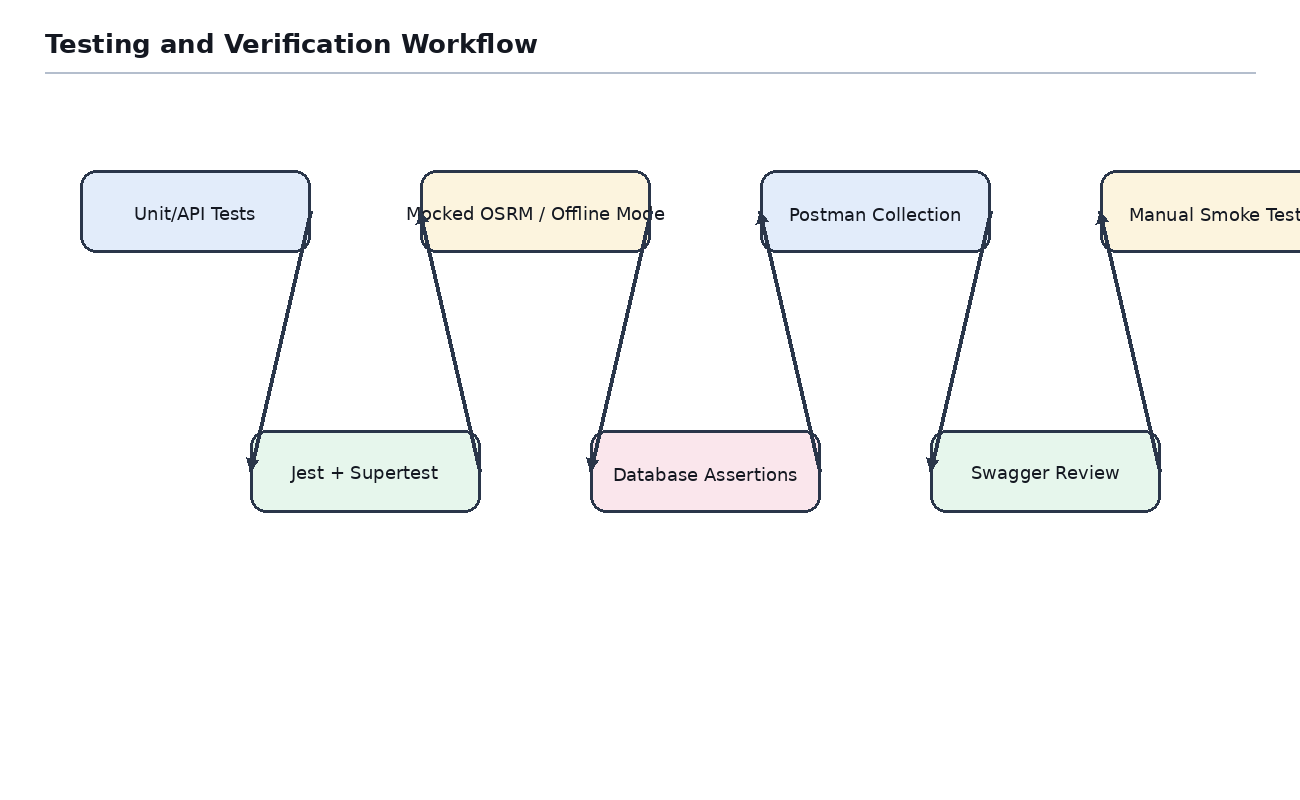
\includegraphics[width=0.84\textwidth]{testing_workflow.png}
\caption{Testing and Verification Workflow}
\end{figure}
\clearpage

\renewcommand{\chapterheader}{CHAPTER 9}
\chapter{Results and Outcomes}
\section{Implemented Project Surface}
The inspected repository shows a broad backend API surface. It includes authentication, organizations, users, businesses, pickup locations, waste categories, drivers, vehicles, vehicle locations, pickups, dispatch, routing, routes, route stops, dashboard, notifications and audit logs. The Swagger UI screenshot confirms that API documentation is available for backend inspection.

\begin{figure}[h!]
\centering
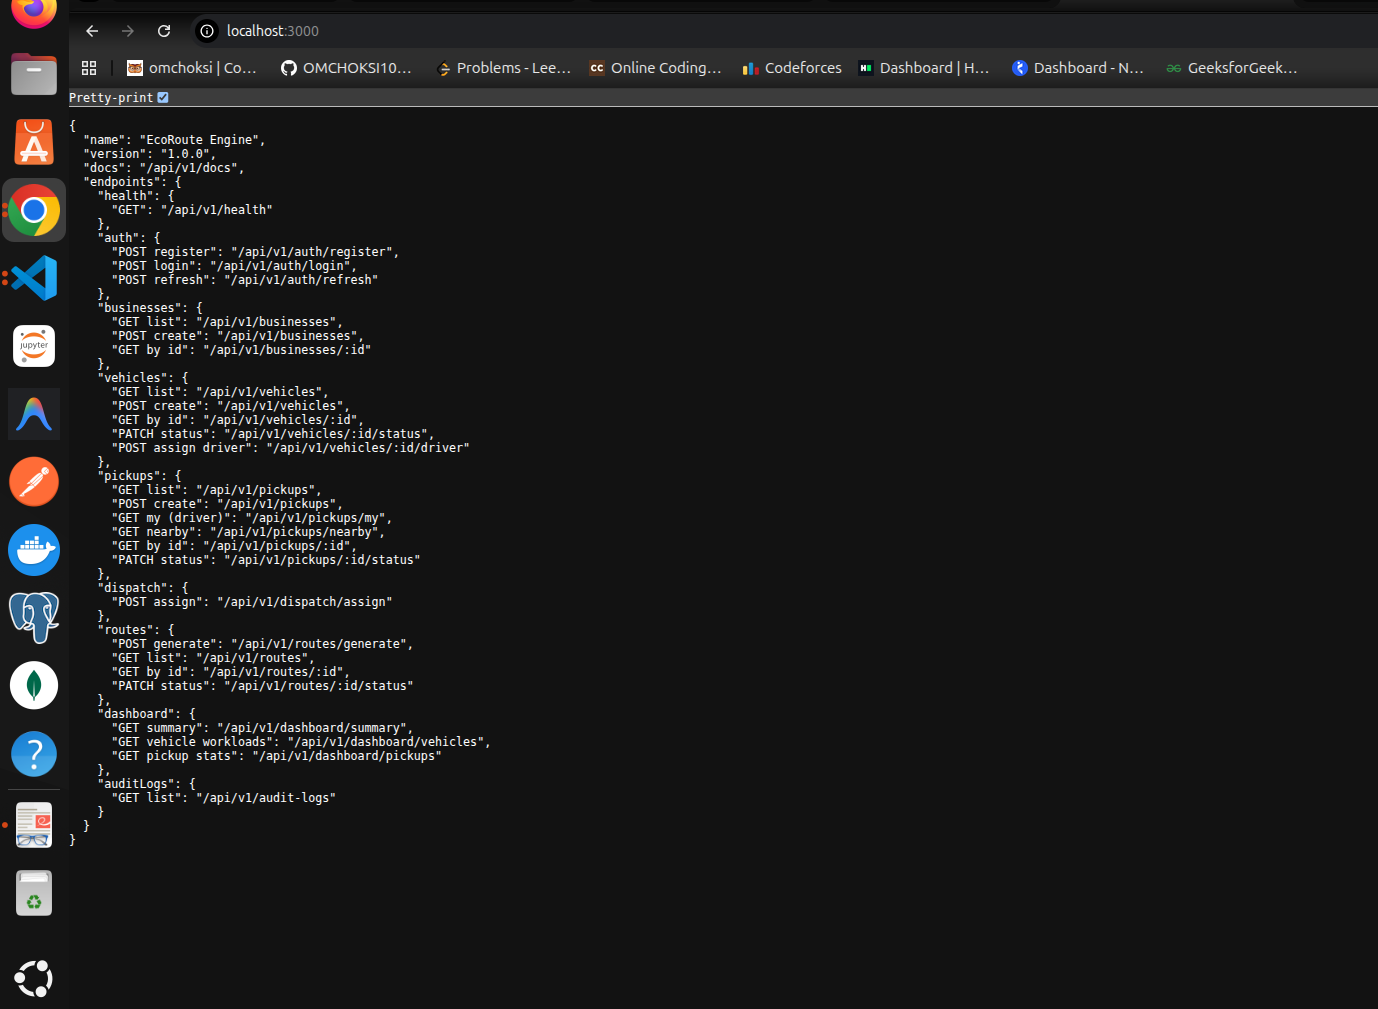
\includegraphics[width=0.86\textwidth]{backend_running.png}
\caption{EcoRoute Backend Running in Development Environment}
\end{figure}

\section{Professional Learning Outcome}
The first month helped me understand how a backend project is documented, structured and tested. I learned how to read existing code, trace a request through layers, understand database migrations, identify security controls and explain architecture using diagrams. This learning will support further work during the remaining five months of internship.
\clearpage

\renewcommand{\chapterheader}{CHAPTER 10}
\chapter{Challenges Faced}
\section{Technical Challenges}
The main technical challenge was understanding how many backend components interact in one project. Authentication, validation, service logic, database constraints, spatial queries, OSRM routing, transactions, audit logs and frontend API hooks are connected. Studying these connections required careful reading of routes, services, repositories and migrations.

\section{Documentation Challenges}
Another challenge was preparing an honest academic report for an ongoing internship. Since only one month has been completed, the report must not overclaim final production deployment or full internship completion. It must clearly state that the internship is six months long and five months are still remaining.

\section{How Challenges Were Addressed}
The challenges were handled by inspecting actual repository files, using screenshots already present in the docs folder, referring to Bhumi's DOCX for academic formatting flow and preparing Mermaid-style diagrams that match the EcoRoute architecture.
\clearpage

\renewcommand{\chapterheader}{CHAPTER 11}
\chapter{Conclusion and Future Scope}
\section{Conclusion}
The first month of my Logicwind internship gave me practical exposure to production-oriented backend development. Through EcoRoute System, I studied a realistic backend involving REST APIs, TypeScript, authentication, RBAC, PostgreSQL/PostGIS, OSRM routing, Docker setup, OpenAPI documentation and automated tests. This experience strengthened my backend foundation as an AIML student because intelligent systems also require reliable backend infrastructure.

\section{Future Scope}
Future scope includes deeper frontend-backend integration, advanced route optimization, richer dashboard visualizations, notification improvements, load testing, production observability, queue-backed dispatch jobs and further GraphQL/Apollo Server learning. The remaining five months of the internship will help me move from guided learning toward more independent backend contribution.
\clearpage

\renewcommand{\chapterheader}{REFERENCES}
\chapter*{References}
\addcontentsline{toc}{chapter}{References}
\footnotesize
\begin{enumerate}
\item EcoRoute Engine repository documentation, \texttt{README.md}, inspected from the local project repository.
\item EcoRoute backend documentation, \texttt{backend/README.md}, inspected from the local project repository.
\item EcoRoute product requirements, \texttt{docs/project.md}, inspected from the local project repository.
\item EcoRoute backend source code, \texttt{backend/src}, inspected from the local project repository.
\item EcoRoute SQL migrations, \texttt{backend/db/migrations}, inspected from the local project repository.
\item EcoRoute frontend source code, \texttt{frontend}, inspected from the local project repository.
\item Docker Compose configuration, \texttt{docker-compose.yml}, inspected from the local project repository.
\item EcoRoute GitHub Repository, \url{https://github.com/OMCHOKSI108/ecoroute-system}
\item Express.js Documentation, \url{https://expressjs.com/}
\item Node.js Documentation, \url{https://nodejs.org/docs/latest/api/}
\item TypeScript Documentation, \url{https://www.typescriptlang.org/docs/}
\item PostgreSQL Documentation, \url{https://www.postgresql.org/docs/}
\item PostGIS Documentation, \url{https://postgis.net/documentation/}
\item Open Source Routing Machine Documentation, \url{https://project-osrm.org/docs/}
\item OpenAPI Specification, \url{https://spec.openapis.org/oas/latest.html}
\item Swagger UI Documentation, \url{https://swagger.io/tools/swagger-ui/}
\item JSON Web Token Introduction, \url{https://jwt.io/introduction}
\item Zod Documentation, \url{https://zod.dev/}
\item Jest Documentation, \url{https://jestjs.io/docs/getting-started}
\item Docker Documentation, \url{https://docs.docker.com/}
\item Apollo GraphQL Documentation, \url{https://www.apollographql.com/docs/}
\item GraphQL Documentation, \url{https://graphql.org/learn/}
\item Mermaid Diagram Syntax Documentation, \url{https://mermaid.js.org/syntax/flowchart.html}
\item CHARUSAT reference report format, the Bhumi reference DOCX, used for logo, front-matter order and academic style reference.
\item Chandubhai S. Patel Institute of Technology, CHARUSAT, \url{https://cspit.charusat.ac.in/}
\end{enumerate}
\normalsize

\end{document}
